\chapter*{Abstract}
This is my abstract.
CEL thesis rules require it to be about 3-5 pages. \todo{This is a todo example}
It is a summary of what you do in your thesis.
Use around 5 pictures and outline whatever you did.
And now a few lines of information.


Polar codes are the first codes to asymptotically achieve channel capacity with low complexity encoders and decoders.
They were first introduced by Erdal Arikan in 2009 \cite{polar:arikan09}.

Channel coding has always been a challenging task because it draws a lot of resources, especially in software implementations.
Software Radio is getting more prominent because it offers several advantages among which are higher flexibility and better maintainability.
Future radio systems are aimed at being run on virtualized servers instead of dedicated hardware in base stations \cite{cloudran:2015}.
Polar codes may be a promising candidate for future radio systems if they can be implemented efficiently in software.

In this thesis the theory behind polar codes and a polar code implementation in GNU Radio is presented.
This implementation is then evaluated regarding parameterization options and their impact on error correction performance.
The evaluation includes a comparison to state-of-the-art \ac{LDPC} codes.


\begin{figure}[!htb]
  \begin{subfigure}[t]{.49\textwidth}
    \begin{center}
      \def\dist{1.5}
      \def\power{3}
      \usetikzlibrary[topaths, calc]

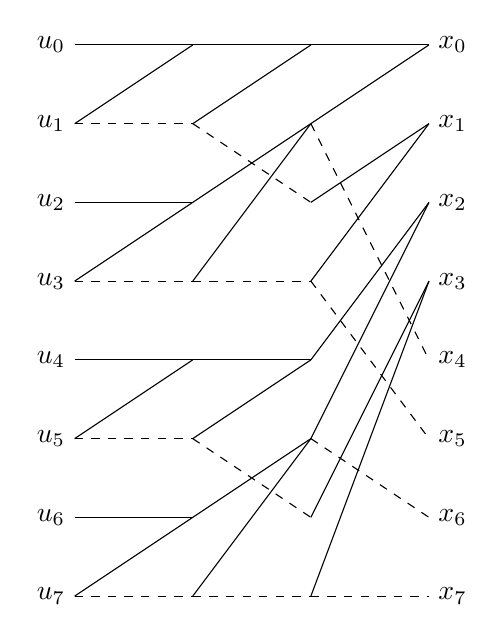
\begin{tikzpicture}[transform shape]
% \def\dist{1.5}
% \def\power{3}
  \pgfmathparse{\power-1}
  \newcount\powerleq
  \let\powerleq\pgfmathresult
  \pgfmathparse{int(2^\power)}
  \newcount\blocksize
  \let\blocksize\pgfmathresult
  \pgfmathparse{\blocksize-1}
  \newcount\blockleq
  \let\blockleq\pgfmathresult

  
  \foreach \j in {0,...,\powerleq}{
    \pgfmathparse{int(\j+1)}
    \let\drow\pgfmathresult
    
    \pgfmathparse{int(2^(\j+1))}
    \let\ccsize\pgfmathresult
    
    \pgfmathparse{int(\ccsize/2)}
    \let\cchalf\pgfmathresult
    
    \foreach \i in {0,...,\blockleq}{
      \pgfmathparse{int(mod(\i,2))}
      \let\n\pgfmathresult
      
      \pgfmathparse{int(\ccsize * int(\i / \ccsize))}
      \let\dblock\pgfmathresult
      
      \pgfmathparse{\dblock + int(mod(\i, \ccsize) / 2) + \cchalf}%(\ccsize * int(\i / \ccsize)) + int(mod(2* (\i + \cchalf), \ccsize)) + 1}
      \let\dest\pgfmathresult
      \path (\dist*\j, \i) edge (\dist*\drow, \dest);
      \ifnum\n=0
	\path (\dist*\j, \i) edge [dashed] (\dist*\drow, \dest-\cchalf);
      \fi
    }
  }
   
  \foreach \i in {0,...,\blockleq}{
    \node[draw=none] at (-0.3, \blockleq-\i) {$u_{\i}$};
    \node[draw=none] at (\dist*\power+0.3, \blockleq-\i) {$x_{\i}$};
  }

\end{tikzpicture}

      \caption{8 bit polar encoder}
      \label{abs:polar_8bit_encoder_natural}
    \end{center}
  \end{subfigure}\,%
  \begin{subfigure}[t]{.49\textwidth}
    \begin{center}
      \def\dist{1.5}
      \def\power{3}
      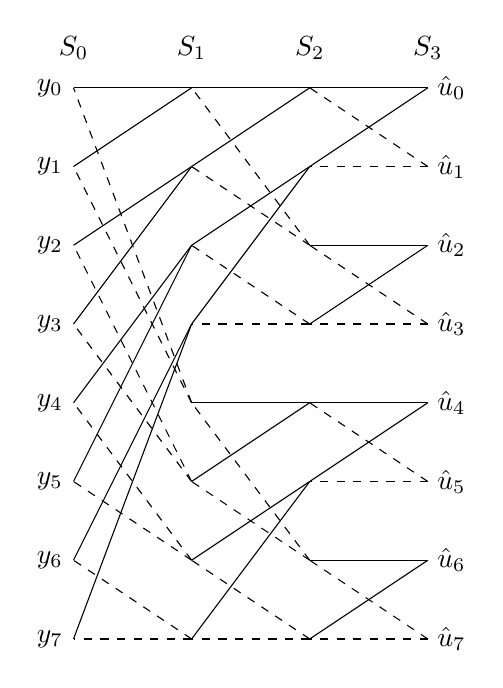
\begin{tikzpicture}[node distance = 1.5cm, auto]
% \def\dist{1.5}
% \def\power{4}
   \pgfmathparse{\power-1}
  \newcount\powerleq
  \let\powerleq\pgfmathresult
  \pgfmathparse{int(2^\power)}
  \newcount\blocksize
  \let\blocksize\pgfmathresult
  \pgfmathparse{\blocksize-1}
  \newcount\blockleq
  \let\blockleq\pgfmathresult
  
  \foreach \j in {0,...,\powerleq}{
    \pgfmathparse{int(-1*\j-1)}
    \let\srow\pgfmathresult
    
    \pgfmathparse{int(-1*\j)}
    \let\drow\pgfmathresult
    
    \pgfmathparse{int(2^(\j+1))}
    \let\ccsize\pgfmathresult
    
    \pgfmathparse{int(\ccsize/2)}
    \let\cchalf\pgfmathresult
    
    \foreach \i in {0,...,\blockleq}{
      \pgfmathparse{int(mod(\i,\ccsize))}
      \let\n\pgfmathresult

      
      \ifnum\n<\cchalf
	\path (\dist*\drow, \i) edge [dashed] (\dist*\srow, \i+\n);
	\path (\dist*\drow, \i) edge [dashed] (\dist*\srow, \i+\n+1);
      \else
	\pgfmathparse{int(\ccsize * int(\i / \ccsize)) + int(mod(2* (\i + \cchalf), \ccsize) )}
	\let\jumpsize\pgfmathresult
	\path (\dist*\drow, \i) edge (\dist*\srow, \jumpsize);
	\path (\dist*\drow, \i) edge (\dist*\srow, \jumpsize+1);
      \fi
    }
  }

  
  \foreach \i in {0,...,\blockleq}{
    \node[draw=none] at (-0.3-\dist*\power, \blockleq-\i) {$y_{\i}$};
    \node[draw=none] at (0.3, \blockleq-\i) {$\hat{u}_{\i}$};
  }
  
  \foreach \i in {0,...,\power}{
    \node[draw=none] at (-1*\dist*\power+\dist*\i, \blocksize-0.5) {$S_{\i}$};
  }

\end{tikzpicture}
      \caption{8 bit polar decoder}
      \label{abs:polar_8bit_decoder}
    \end{center}
  \end{subfigure}%
  \caption{Polar code encoding and decoding}
  \label{abs:encoder-decoder}
\end{figure}

The polar encoder is shown in Fig. \ref{abs:polar_8bit_encoder_natural}.

